\problem{What is an ideal and practical filter? Mention the applications of filters with suitable
examples.}
An ideal filter is one that has unity gain $(H=1)$ in the passband and zero gain $(H=0)$ in the stop band. In other words, the passband attenuation is zero $(\alpha=0)$ and stopband attenuation is infinite $(\alpha\rightarrow\infty)$. This means that the transition between the passband and stopband is sharp and the response is called a brick-wall response due to its sharp shape.
\begin{figure}[H]
    \begin{subfigure}{0.48\textwidth}
        \centering
        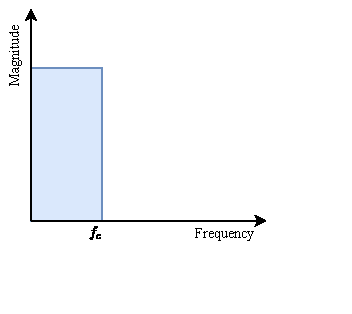
\includegraphics[width=0.7\linewidth]{../Figures/idealized_lp}
        \caption{Lowpass filter response}
        \label{fig:ideal-a}
    \end{subfigure}
    \begin{subfigure}{0.48\textwidth}
        \centering
        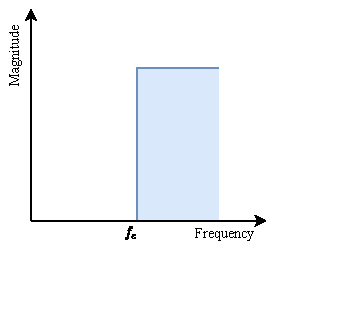
\includegraphics[width=0.7\linewidth]{../Figures/idealized_hp}
        \caption{Highpass filter response}
        \label{fig:ideal-b}
    \end{subfigure}\newline
    \begin{subfigure}{0.48\textwidth}
        \centering
        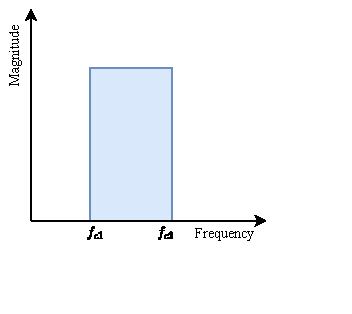
\includegraphics[width=0.7\linewidth]{../Figures/idealized_bp}
        \caption{Bandpass filter response}
        \label{fig:ideal-c}
    \end{subfigure}
    \begin{subfigure}{0.48\textwidth}
        \centering
        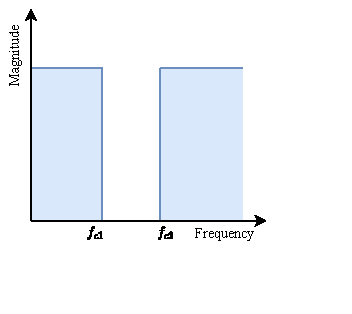
\includegraphics[width=0.7\linewidth]{../Figures/idealized_bs}
        \caption{Bandstop filter response}
        \label{fig:ideal-d}
    \end{subfigure}
    \caption{Ideal filter responses}
    \label{fig:ideal}
\end{figure}
The responses for different filters shown in Figure~\ref{fig:ideal} are not practically achievable since the system to produce such response need to be non-causal, which is not possible to realize.
\\A practical filter is one that does not have unity gain $(H\neq1)$ in the passband and non-zero gain $(H\neq0)$ in the stop band. In other words, the passband attenuation has some attenuation and the stopband has a small value of attenuation. The transition between the passband and stopband is not sharp, rather a gradual decay is seen in the transition band.
\begin{figure}[H]
    \begin{subfigure}{0.48\textwidth}
        \centering
        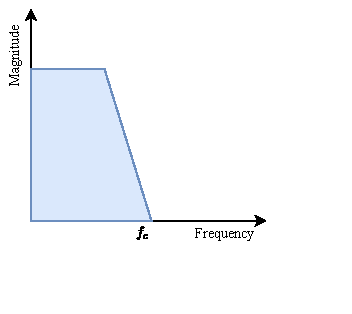
\includegraphics[width=0.7\linewidth]{../Figures/practical_lp}
        \caption{Lowpass filter response}
        \label{fig:practical-a}
    \end{subfigure}
    \begin{subfigure}{0.48\textwidth}
        \centering
        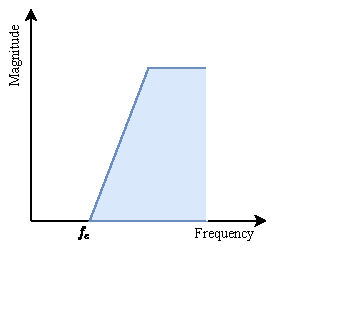
\includegraphics[width=0.7\linewidth]{../Figures/practical_hp}
        \caption{Highpass filter response}
        \label{fig:practical-b}
    \end{subfigure}\newline
    \begin{subfigure}{0.48\textwidth}
        \centering
        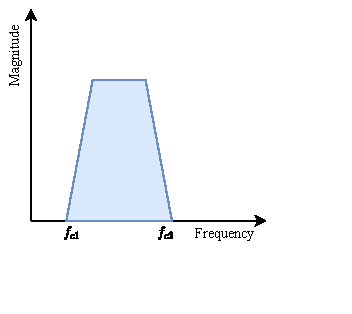
\includegraphics[width=0.7\linewidth]{../Figures/practical_bp}
        \caption{Bandpass filter response}
        \label{fig:practical-c}
    \end{subfigure}
    \begin{subfigure}{0.48\textwidth}
        \centering
        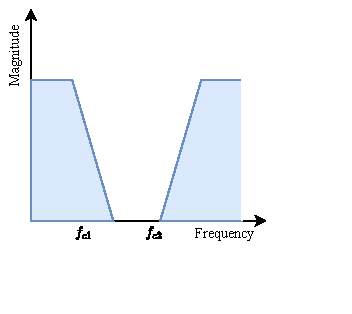
\includegraphics[width=0.7\linewidth]{../Figures/practical_bs}
        \caption{Bandstop filter response}
        \label{fig:practical-d}
    \end{subfigure}
    \caption{Practical filter responses}
    \label{fig:practical}
\end{figure}

However, the responses for different filters shown in Figure~\ref{fig:practical} are not the true form that they exist in. The flat passband shown in the responses can have attenuation ripples. Similarly, the transition in reality, is not a straight line and there may exist ripple in the stopband as well. For a general lowpass filter, the response takes the form shown in Figure~\ref{fig:practical-true}.
\begin{figure}[H]
    \centering
    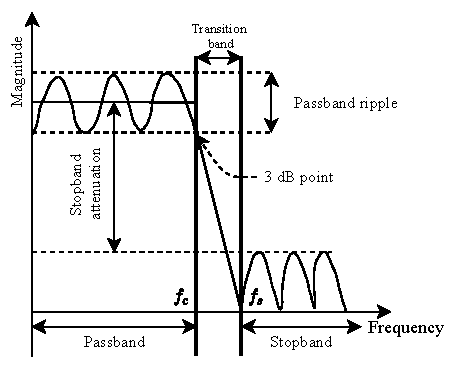
\includegraphics[scale=1.2]{../Figures/practical}
    \caption{Actual practical response of a lowpass filter}
    \label{fig:practical-true}
\end{figure}

The applications of filters are listed below:
\begin{enumerate}
    \item Filters are an important component in frequency domain analysis of a signal.
    \item Filters are used in various audio systems for pre-amplification and equalization. They are also used in multi-way loudspeakers to distribute different audio frequencies to different speakers for tone control.
    \item Filters are used in image frequency rejection in radio, television and satellite receivers.
    \item During telephone communication, filters are used to suppress background noise.
    \item Filters are used for satellite communication where the used carrier signal is analog in nature.
\end{enumerate}